\section{Calibration Production and Application} \label{sec:calibration-production}
% former label: sec:processing:calibration

Each subsection will describe the calibration product, its construction algorithm, and the corresponding ISR correction task.
We may also include a table of the data product and the name of the associated calibration task.
Figure~\ref{fig:calib-dependency} summarizes calibration-product dependencies.
The integrative ISR pipeline for DP2 science data, including the order in which corrections are applied (Figure~\ref{fig:isr-pipeline}), is described in \S\ref{sec:isr-science}.

\begin{figure}[t!]
    \centering
    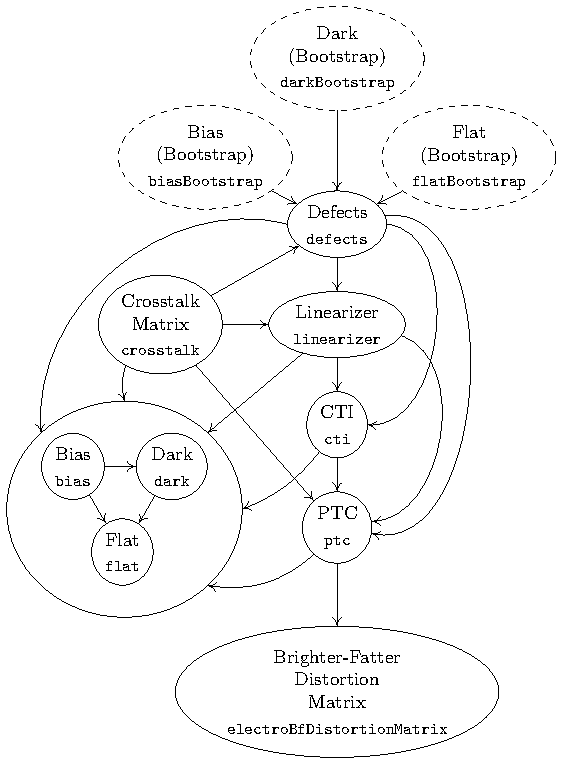
\includegraphics[width=\columnwidth]{figures/calib-dependency.pdf}
    \caption{Calibration production dependency graph.
    Arrows indicate data or dependency flow (``x $\rightarrow$ y'' means ``y depends on x'').
    Solid outlined boxes represent datasets that are deployed/released with data products while dashed boxes represent internal or intermediate datasets that are not formally released to users.}
    \label{fig:calib-dependency}
\end{figure}

% NOTE: order follows calib-dependency figure

\subsection{Curated Calibrations} \label{sec:processing:calibration:curated-calibs}

\subsection{Auxiliary Data Products} \label{sec:processing:calibration:auxiliary-data-products}

\subsection{Crosstalk} \label{sec:processing:calibration:xtalk}
Describe how the crosstalk matrices are constructed.

\subsection{Defects} \label{sec:processing:calibration:defects}

We build a \textsc{defects} calibration product based on defects manually defined and automatically detected.
They correspond to pixels which output is not well corrected by our ISR approach.
These Defect pixels are masked and marked as \textsc{BAD} for the downstreamed analysis and interpolated over for visual inspection.

The \textsc{defects} calibration product is constructed by measuring defects on bias, dark, flats and then merged together.
The defects detection consist of the following steps:
\begin{itemize}
    \item correct for the gradient across the focal plane, by applying a gradient correction to each amplifiers
    from the gradient measured in a binned image.
    \item a background estimate is done and removed,
    \item hot pixels as defined as pixels with more than 5 e-/s (scaled by the exposure time) of dark current, above 1000 ADU in bias are measured,
    \item cold pixels as defined as pixels with photoresponse less than $80\%$ of the flat mean are measured,
    \item pixels along the midline break (the interface between the top and bottom amplifiers) in E2V detectors are
    set to the median of the flats (so they are not found by the defect code),
    \item bad columns masking.
\end{itemize}

Afterwards, these measured defects are merged together, and the edges of the detectors are masked, to
mask the so-called picture frame effect corresponding to the presence of large electric field at the edges of the CCDs.

For DP2, these defects were produced by using 'bootstrap' version of the bias, dark, flat as these calibration products need the defects themselves to be defined.
This will probably be updated in future iteration of calibration products.

Additionally manual defects are large features present in LSSTCam detectors, such as the large defect in detector 0
which induces large bleeds. LSSTCam manual defects are defined in \url{https://github.com/lsst/obs_lsst_data/tree/main/lsstCam/manual_defects}.
%We describe how defect masks are generated (bad pixels/columns, saturation trails, and other artifacts), the thresholds used, and how masks are combined across exposures.

Further defect statistical analyses, description of the defect monitoring, masking optimization are postponed to a future paper.
Additional masking is applied to an exposure in the ISR processing, as described in Sec ??.

\subsection{Non-Linearity} \label{sec:processing:calibration:linearity}

Non-linearity (NL) describes a deviation from simple proportionality when mapping amplified voltage integrated during readout to the number of analog-to-digital units (ADU) or counts.
Non-linearity is signal-dependent and is often not a simple function of signal level; it can change suddenly above a large signal level that is characteristic to each readout amplifier; and it can drift with sensor temperature and with time, as slow electronic shifts in the bias level accumulate over a long calibration campaign.
In practice it introduces pixel-level measurement bias (up to x\% from the true signal) and invalidates Poisson counting statistics and can interfere with measurement of gain (which shouldn't change or drift with signal level).
Correcting NL to better than y\% is therefore a prerequisite for reliable downstream calibration products and science analyses.

We can measure non-linearity by measuring the response of pixel values to a change in illumination level.
The in-dome calibration illumination system can deliver an approximately uniform flux of light across the LSSTCam focal plane.
Given a known change in some input illumination level, we should be able predict a change in the number of counts in an image, which we can then compare to the measured change counts.

We do not have independent measurements of the photodiode current produced by our calibration illumination system that we can integrate of the exposure time and use as a baseline truth of the amount of incident light while taking an exposure.
The exposure time, which is precisely measured, makes a natural proxy for missing photodiode measurements.
We therefore calibrate NL by fitting a relation between exposure time ($\Delta t$, abscissa) and the mean measured flat-field signal ($\mu$, ordinate).

We measured $543\times2$ flat field exposures at evenly spaced illumination levels. We went as low as 100~analog-to-digital units (ADU) and continued beyond pixel saturation.
At each illumination level, a pair of flats was acquired by varying both photodiode current and exposure time to achieve the targeted levels, measuring the mean signal level as $\mu_i = \mathrm{avg}(F_i^{(1)},F_i^{(2)})$~(in ADU).
These data were acquired with illumination levels decided in random order to decouple signal-dependent non-linearity and time-dependent drifts in non-linearity.

\begin{figure}[t]
    \centering
    % TODO: add exposure-time vs.\ mean-signal figure asset
    \fbox{\parbox{0.75\columnwidth}{\centering\vspace{1.5in}\small\textit{Figure pending}\vspace{1.5in}}}
    \caption{Mean flat-field signal as a function of exposure time for a representative amplifier.
    Discontinuities at LED current-setting boundaries partition the data into distinct illumination groups.}
    \label{fig:linearity-exptime-vs-signal}
\end{figure}

Figure~\ref{fig:linearity-exptime-vs-signal} shows the resulting relation for a representative amplifier.
Discontinuities appear at the boundaries between LED current settings, producing different signal levels for the same exposure time.
These data are partitioned into groups associated with distinct LED illumination settings.
Grouping is determined by computationally searching for jumps in the ratio of mean detector signal to exposure time or via exposure metadata.
Within each group we allow a distinct proportionality constant $k_j$ to capture the size of the jumps.

To first order, the trend between exposure time and the mean measured flat-field signal over properly scaled groups is linear and related to the intrinisc gain in each readout channel.
We can fit a simple slope and intercept to this trend to the low signal points; the highest signal level in each channel above which this approximation break is the ``linearity turnoff" (as indicated in Figure~\ref{fig:linearity-turnoff}).
Points above the turnoff are excluded from the NL fit because there is a maximum signal above which the measured counts can no longer be trusted due to hardware limitations at the output of the detector (Figure~\ref{fig:detector-boxes}).

\begin{figure}[t]
    \centering
    % TODO: add linearity turnoff figure asset
    \fbox{\parbox{0.75\columnwidth}{\centering\vspace{1.5in}\small\textit{Figure pending}\vspace{1.5in}}}
    \caption{Linearity turnoff for a representative amplifier.
    The turnoff marks the highest signal level below which the exposure-time-to-signal relation remains approximately linear.}
    \label{fig:linearity-turnoff}
\end{figure}

The NL model we fit to this relation is an extension of the formalism developed by \citet{astier-2019}.
We represent the deviation from linearity by an Akima spline $S(\mu)$ of the measured mean signal $\mu$.

For each exposure $i$ in group $j$ we define the residual ratio
\begin{equation}
    r_i = \frac{\mu_i - S(\mu_i) - O}{k_j\, D_{i}}
    \label{eq:spline-nl-fit}
\end{equation}
where $D_{i}$ is the data used for the abscissa (exposure time), $O$ is an optional constant offset that absorbs scattered light or other signal not proportional to $D_{i}$, and $w_i$ are weights.

The fit minimizes a uniformly weighted ($w_i = 1$) least-squares objective over all accepted points:
\begin{equation}
    \chi^2 = \sum_{i} w_i \left(r_i - 1\right)^2. \label{eq:linearity-chisq}
\end{equation}
The fit is subject to the boundary conditions $S(0) = 0$ and $\langle S(\mu)\rangle = 0$ over the fit range.
The first constraint fixes the origin such that zero illumination is always measured zero measured signal; the second ensures that the spline captures deviations from linearity independently from knowning the true amplifier gain.

In addition, any hardware sensitities are absorbed by nuisance parameters that we parameterize as 1st order linear corrections to $\mu$ before the spline is evaluated:
\begin{align}
    \mu &\rightarrow \mu \left(1 + \alpha\, T_i\right), \label{eq:linearity-temp} \\
    \mu &\rightarrow \mu \left(1 + \beta\, t_i\right), \label{eq:linearity-time}
\end{align}
where $T_i$ is a readout temperature (referenced to the median over the campaign), $t_i$ is the Modified Julian Date (MJD) of the midpoint of the shutter open time, and $\alpha$ and $\beta$ are fitted coefficients that describe each sensitivity.
For LSSTCam DP2 calibration production we fit both the temperature and temporal coefficients as well as the scattered-light offset $O$ on the spline.

We could perform this fit independently for every amplifier on every detector. However, most of the non-linearity is common to all amplifiers due to similar readout architectures, with only small amplifier-to-amplifier variations on top that.
In addition, each independent fit to every amplifier would pick up not just the intrinsic non-linearity in amplifiers, but also exposure-to-exposure spatial illumination variation that occurs during the calibration campaign.
To better characterize this, it makes since to perform a spline fit on each amplifier relative to both a single reference exposure and a reference amplifier on the same detector.

We can distinguish an \emph{absolute} non-linearity in a single reference amplifier on a detector and the \emph{relative} non-linearity of other amplifiers to that reference amplifier, the process for which is summarized in Algorithm~\ref{alg:linearity-double-spline}.
After choosing a reference amplfier and a reference exposure, we do (1) a relative spline fit on every other amplifier using  the variation of its mean flat-field signal $\mu$ relative to the reference amplifier and to the $\mu$ in a single reference exposure, and then (2)
an absolute spline fit on the reference amplifier using the usual from $\mu$ versus $\Delta t$.
Every amplifier on a detector has a shared absolute spline fit based on the reference amplifier for that detector and a relative spline fit computed relative to a reference amplifier and a reference exposure ($S_{\mathrm{rel}}(\mu) = 0$ for the reference amplifier).

\begin{algorithm}[H]
\caption{Double-spline linearity fit (single detector)}
\label{alg:linearity-double-spline}
\begin{algorithmic}[1]
\For{each amplifier $a$}
    \State $k_j \leftarrow$ \Call{Find Groups}{$\mu_a$, $\Delta t$}
    \State \Call{Compute linearity turnoff}{$\mu_a$, $\Delta t$}
\EndFor
\State choose reference amplifier $\mathrm{ref}$ with the highest linearity turnoff
\State choose reference exposure $i_0$, the flat whose mean signal $\mu_{\mathrm{ref}} = 10^4$ on amplifier $\mathrm{ref}$ is nearest the target signal level
\For{each exposure $i$}
    % \State compare flat $i$ to the reference exposure $i_0$
    % \State $\mu_{\mathrm{ref},i} \leftarrow$  $\mu_{\mathrm{ref}}$ / $\mu_{\mathrm{ref}, i_0}$ % mean signal on amplifier $\mathrm{ref}$ in exposure $i$, normalized to $i_0$
    \For{each amplifier $a \neq \mathrm{ref}$}
        \State $D^{\mathrm{rel}}_{i} \leftarrow \mu_{\mathrm{ref}, i} \times (\mu_{a,i_0} / \mu_{\mathrm{ref}, i_0})$  (Relative Abscissa) % mean signal on amplifier $a$ in exposure $i$, normalized to $i_0$ and expressed relative to $\mu_{\mathrm{ref},i}$
        \State $\mu^{\mathrm{rel}}_{i} \leftarrow \mu_{a,i}$ (Relative Ordinate)
    \EndFor

    \State $D^{\mathrm{abs}}_{i} \leftarrow \Delta t_i$ (exposure time)
    \State $\mu^{\mathrm{abs}}_{i} \leftarrow \mu_{\mathrm{ref},i}$ (measured counts)
\EndFor

\Statex \Comment{Spline fit}
\State $S_{\mathrm{abs}}(\mu), O, \alpha, \beta \leftarrow$ \Call{Minimize}{Equation~\ref{eq:linearity-chisq}, $D^{\mathrm{abs}}_{i}$, $\mu^{\mathrm{abs}}_{i}$, $k_j$}
\State $S_{\mathrm{rel}}(\mu) \leftarrow$ \Call{Minimize}{Equation~\ref{eq:linearity-chisq}, $D^{\mathrm{rel}}_{i}$, $\mu^{\mathrm{rel}}_{i}$, $k_j$}
\end{algorithmic}
\end{algorithm}

To determine the corrected mean signal level, we can interpolate the Akima splines to compute a correction: $\mu' = \mu - S_{\mathrm{rel}}(\mu) - S_{\mathrm{abs}}(\mu)$.

If each amplifier is properly linearized around its true gain, we should observe in every exposure that the illumination level is coherent between amplifiers and detectors.
If the linearization is miscalibrated or biased (either because exposure time is not a good proxy for the true integrated photodiode or if constraining $\langle S(\mu)\rangle = 0$ is biased), the amplifiers and detectors will show signal-dependent fractional offsets in mean signal levels in each flat similar to a mis-estimation of gain.

We can check this how the linearized mean signal levels deviate from an overall linear relation over some set of detectors in a given exposure:
For each exposure $i$, we form the linearized signal, $\mu'_i$, on the reference amplifier on every detector and compute the fractional residual:
\begin{equation}
    r_i = \frac{\mu'_i - m_i D_{i}}{y_i},
\end{equation}
where $m_i$ is the slope of a linear fit to $\mu'_i$ versus $D_{i}$.
We take the median $\langle r \rangle_i$ over a subset of focal-plane detectors (in the center of the focal plane) in that exposure and derive a multiplicative correction
\begin{equation}
    N_i = \frac{1}{1 - \langle r \rangle_i},
\end{equation} that we use to rescale the abscissa ($D_{i} \rightarrow N_i D_{i}$) and enforce that the linearization produces a coherent illumination across all detectors.

We can then re-compute the double-spline fit with the normalized abscissa on the reference amplfier. We can repeat the cycle (normalize, spline, normalize, etc.) recursively several times, each time computing the normalization as \begin{equation}
    N_i = \frac{N_i^{\mathrm{prev}}}{1 - \langle r \rangle_i}.
\end{equation}

By including constraints from the whole focal plane, we get to take advantage of the added statistical information.
After one iteration, this gives us a factor of Nx improvement in precision, with added value dropping rapidly after two iterations.

In ISR, given an image with pixel values measured in counts ($F_{ij}$), the final spline model can be interpolated, providing a continuous map from measured counts to the corrected counts for any pixel value within the range of 0 signal to the linearity turnoff, computed as:
$F_{ij}' = F_{ij} - S_{\mathrm{rel}}(F_{ij}) - S_{\mathrm{abs}}(F_{ij})$.

% During science ISR, the linearizer is applied at the non-linearity correction step in Figure~\ref{fig:isr-pipeline}; see \S\ref{sec:isr-science}.


\subsection{Deferred Charge} \label{sec:processing:calibration:cti}

Several distinct effects in the readout chain displace charge from its pixel of origin and leave correlated structure in the serial overscan: (1) a pixel-to-pixel fractional loss during charge transfer referred to as ``global CTI'', (2) a local electronic-offset hysteresis in the output amplifier that mimics deferred charge in the first few overscan columns, and (3) localized capture and delayed release of charge by isolated trap sites in the serial register.
Strictly, only global CTI is ``charge transfer inefficiency'' in the textbook sense, but because all three enter at the same point in the photon transfer chain (Figure~\ref{fig:detector-boxes}) and produce overlapping signatures in the serial overscan, we model them together and produce a single calibration data product that we loosely refer to as ``CTI'' in Figure~\ref{fig:calib-dependency}.
These effects are measured, modeled, and corrected together using the extended pixel edge response (EPER) estimator developed for LSSTCam by \citet{snyder2021}.

Calibrating deferred charge uses the same input data as the linearity dataset (\S\ref{sec:processing:calibration:linearity}), estimating the residual charge in electrons left in the overscan region after integrating and reading out flat field images over a wide range of signal levels.
The global CTI is quantified by a unitless fraction, but the trap size and the electronic drift-scale all carry signal-dependent physical units, so an imperfect conversion from counts back to physical electrons biases the eventual correction.
This calculation therefore needs to happen in native electron units, so we need to remove signal-dependent non-linearities that occur when the signal is measured as counts and estimate a gain conversion from counts to electrons.
For each input exposure, we apply an intermediate pass of instrument signature removal that applies defect masking and non-linearity correction, and converts pixel values to electrons, and also measures the overscan EPER statistics for each readout channel.

The natural way to convert from counts to electrons is to use the gain inferred from the PTC (\S\ref{sec:processing:calibration:ptc}), but the PTC needs to be CTI-corrected to get the most accurate inferred gains, creating what seems like a circular dependency between CTI and PTC calibration production.
We break the cycle by bootstrapping. We create a temporary (intermediate) PTC that is not CTI-corrected, which we fit (see \S\ref{sec:processing:calibration:ptc}) to derive an initial rough estimate of the per-amplifier gain.
That estimate is stored and applied during the ISR of the flat field images before calculating the EPER statistics.
We find that the gains from a PTC without CTI correction are close enough to the final gains measured from a fully calibrated PTC (typically within 1\% of the true gains).
At this level, the rough gains are accurate enough for CTI calibration. The global-CTI fit is unit-free and so insensitive to any gain error, and the trap and local-offset amplitudes have only weak sensitivity to the few-percent gain bias that remains in the bootstrap estimate.

An example of the measured serial EPER statistics as a function of signal level for a single channel readout is shown in Figure~\ref{fig:cti-serial-eper}.
The global CTI produces an overall offset of this curve at all signal levels, the electronic offset produces a linear slope in the curve as a function of signal level, and the serial traps produce non-linear jumps that ``turn on'' above some signal level after a trap fills up and begins releasing charge with a characteristic timescale.
There is a point at high signal levels at which we can no longer effectively transfer charge pixel to pixel, which we define as the ``serial CTI turnoff'' as indicated in the figure.
We calculate this point as the highest mean signal for which the serial EPER remains consistent with a sigma-clipped linear fit to the low-signal points. For the majority of readout channels, the image region flat field level was not high enough to observe a serial CTI turnoff, which we then set as the maximum observed signal level.

\begin{figure}[t]
    \centering
    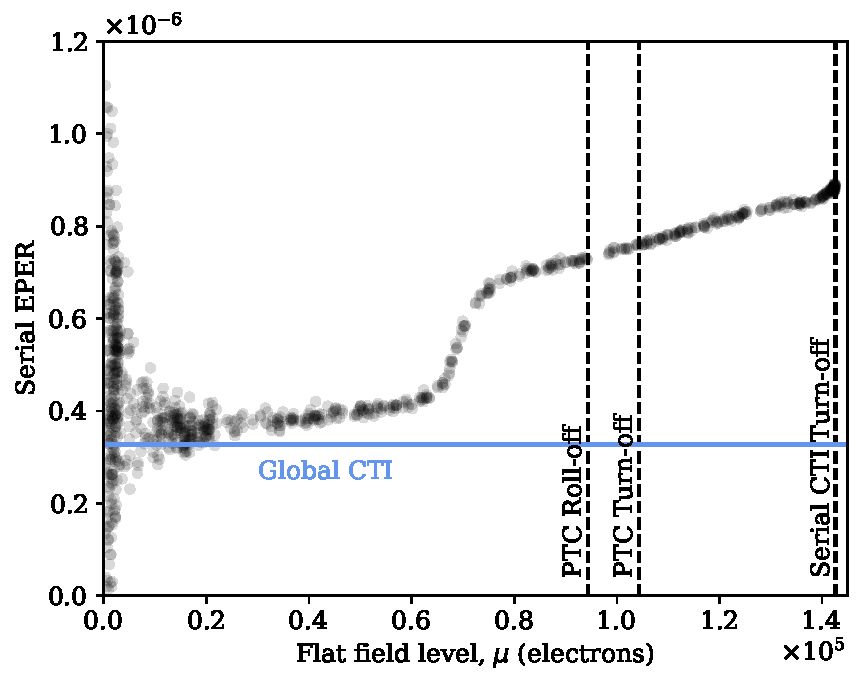
\includegraphics[width=\columnwidth]{figures/cti-det93-ampC04-serial-eper.pdf}
    \caption{Serial EPER statistics as a function of flat-field signal level for detector/amplifier R22-S10/C04.
    Vertical markers indicate the PTC rolloff and turnoff thresholds (described in \S\ref{sec:processing:calibration:ptc}) and the serial CTI turnoff derived from the low-signal trend.
    The global CTI fit produces the overall offset of the measured curve at all signal levels.}
    \label{fig:cti-serial-eper}
\end{figure}

The CTI solver simulates charge readout and each of the three effects at the amplifier image level for a given set of parameters.
The model in the simulation is parameterized by a global serial CTI parameter $b$ that is a fractional charge loss per pixel transfer, a local electronic offset described by drift scale $A_L$ and decay time $\tau_L$, and a spline-based serial charge-trap decay model whose size is allowed to depend on the signal in the last imaging column.
We perform a least squares fit that finds the optimal set of parameters that can reproduce the measured overscan statistics trend as a function of signal level.
Then the solver fits these parameters to the overscan image in stages.
First, it varies only the local offset parameters, then the global CTI parameter, and then the trap capture curve from residuals between model and data.
Exposures above configured flux limits are excluded from each stage (typically $10^4$~electrons for the global CTI fit and $1.5\times10^5$~electrons for trap fitting).

The LSST Science Requirements Document requires that total deferred charge measured by EPER be kept under a total of $5\times10^{-6}$ for signal levels below saturation level on each amplifier (citation needed).
Within the population of amplifiers in active science detectors, only 95 amplifiers do not meet this requirement without ISR correction.
Figure~\ref{fig:cti-global-histogram} shows the distribution of inferred global CTI across all amplifiers on the LSSTCam focal plane, and we show that 26 have a global CTI offset that is already above the maximum allowed threshold.
The majority of these (19) are bad amplifiers that are in the detector corners (C00, C07, C10, C17) positioned near the serial register, and it is possible that what is inferred as global CTI could be a serial trap that turns on at very low signal levels (below the $10^4$ electron level) and appears as an overall offset that is mistaken for global CTI.

\begin{figure}[t]
    \centering
    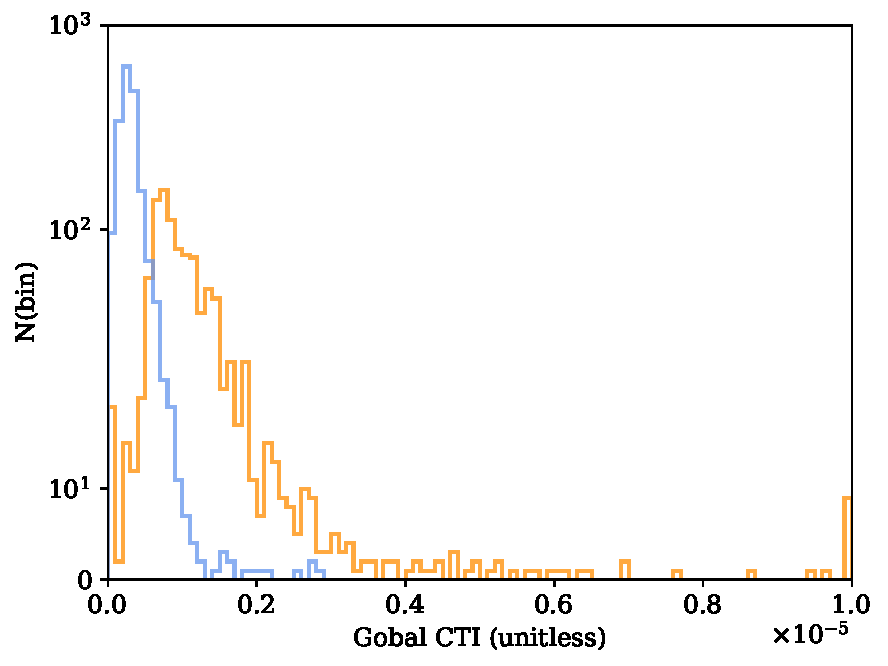
\includegraphics[width=\columnwidth]{figures/cti-det93-ampC04-global-cti-histogram.pdf}
    \caption{Distribution of inferred global serial CTI across all science sensor amplifiers on the LSSTCam focal plane.
    \textit{Blue}---Teledyne e2v (E2V) detectors; \textit{Orange}---Imaging Technology Laboratory (ITL) detectors.
    The fit to the deferred charge model allows global CTI to vary up to $1.0 \times 10^{-5}$.}
    \label{fig:cti-global-histogram}
\end{figure}
% TODO: Add CTI-corrected versions of Figure~\ref{fig:cti-global-histogram}.

When correcting deferred charge from an image during ISR, the deferred-charge correction takes in these fit parameters and applies the inverse operators from the model.
The global CTI and local-offset fits, and the inverse correction operators applied during ISR, are the same for both ITL and E2V sensors, but serial traps are fitted only on ITL since it was observed that E2V sensors had small trap size that was difficult to measure beyond noise fluctuations and already negligible enough not to require correction.
After applying a deferred charge correction, we can re-compute the EPER statistics on the corrected dataset and find that all amplifiers meet the science requirements.

While there can be deferred charge from a charge transfer in the parallel direction (shift row-to-row), in principle this is a difficult quantity to estimate accurately from parallel overscan statistics.
EPER statistics computed in the parallel overscan region are noisy and reveal no statistically significant charge residuals, so we do not apply any parallel deferred charge correction to science images.

% During science ISR, this product is applied at the deferred-charge correction step in Figure~\ref{fig:isr-pipeline}; see \S\ref{sec:isr-science}.


\subsection{Photon Transfer Curve (PTC)} \label{sec:processing:calibration:ptc}

The photon transfer curve (PTC) characterizes how pixels respond to varying signal levels in a given wavelength band by measuring covariances between pixels in flat field exposures across a range of illumination levels.
This dataset provides critical calibration information including amplifier-level read noise and gain for variance plane estimation, saturation thresholds for masking, and parameters needed to correct for non-linearity, charge transfer inefficiency (CTI), and the brighter-fatter effect.
All of these parameters can differ at the amplifier level.

% The photon transfer curve used to calibrate LSSTCam for DP2 is measured from $543\times2$ flat field exposures at evenly spaced illumination levels as low as 100~analog-to-digital units (ADU) and reaching at least 10\% beyond saturation.
% At each illumination level, a pair of flats was acquired by varying both LED output and exposure time to achieve the target signal.
% We measure the covariance between pixels on the difference image of the two exposures to remove variations sourced by static, fixed-pattern artifacts.

Let $F_1$ and $F_2$ denote the two flats at a given illumination level, and let $\mu = \mathrm{avg}(F_1,F_2)$ denote the mean signal level (in ADU) over the image and away from the detector edges.
The covariance between a pixel $\mathbf{x}=(0,0)$ and a neighbor at pixel $\mathbf{x}'=(i,j)$ is:
\begin{equation}
    C_{ij} \;=\; \tfrac{1}{2}\,
    \mathrm{Cov}\!\left(F_1(\mathbf{x})-F_2(\mathbf{x}),\,
                       F_1(\mathbf{x}')-F_2(\mathbf{x}')\right).
\end{equation}

% Following the standard front-illuminated CCD convention, serial (row) readout proceeds along $(1,0)$ and parallel (column) readout along $(0,1)$.

\paragraph{Pre-model fit}
Preliminarily, we fit only the variance to an approximate exponential relation derived in \citet{astier-2019} (their Eq.~16).
\begin{equation}
    C_{00}^{\mathrm{exp.\,approx}}(\mu) = \frac{1}{2 g^2 a_{00}}\bigl[\exp(2 a_{00} \mu g) - 1\bigr] + \frac{n_{00}}{g^2}\ .
\end{equation}
In this expression, covariances are contributed by a gain $g$ (electrons$/\mathrm{ADU}$), noise pedestal $n_{00}$ (electrons$^2$), and a single brighter-fatter coefficient $a_{00}$ ($1/$electrons) which has the effect of decreasing the image variance.

Near saturation, the variance deviates from this functional form, exhibiting a gradual rollover rather than a sharp cutoff due to electrostatic effects that are difficult to model analytically.
On top of the exponential approximation, we introduce an empirical saturation term:
\begin{equation}
    C_{00}^{\mathrm{sat}}(\mu) = \left\{
        \begin{array}{ll}
            -e^{-(\mu-\mu_0)/\tau} & \mu \ge \mu_0 \\
            0 & \mu < \mu_0
        \end{array}
    \right.,
\end{equation}
where $\mu_0$ marks the onset of the PTC ``rolloff'' effects and $\tau$ controls the shape of the rollover.
The total preliminary fit model is $C_{00}^{\mathrm{prelim.}}(\mu) = C_{00}^{\mathrm{exp.\,approx}}(\mu) + C_{00}^{\mathrm{sat}}(\mu)$ to the unweighted points. This fit is performed iteratively with additional 3~sigma clipping until convergence.
The ``PTC turnoff'' is defined as the signal level of the last unmasked point following the fit to only the exponential approximation, typically corresponding to the maximum of the variance curve and generally higher than the rolloff threshold.
The ``PTC rolloff'' is the signal level where $C_{00}^{\mathrm{prelim.}}(\mu)$ and $C_{00}^{\mathrm{exp.\,approx}}$ deviate by more than 1\%.

\paragraph{Final model fit}
With the remaining points below the PTC rolloff, we fit the complete covariance expansion from \citet{astier-2019} (their Eq.~20):
\begin{equation}
    \begin{aligned}
    C_{ij}^{\mathrm{model}}(\mu) = \frac{\mu}{g} \Bigl[ \delta_{i0}\delta_{j0}
      &+ a_{ij}\mu g \\
      &+ \frac{2}{3}\left([\mathbf{a}\otimes\mathbf{a} + \mathbf{ab}]_{ij}\right)(\mu g)^{2} \\
      &+ \frac{1}{6}\left(2\mathbf{a}\otimes\mathbf{a}\otimes\mathbf{a} + 5\mathbf{a}\otimes\mathbf{ab}\right)_{ij}(\mu g)^{3} \\
      &+ \mathcal{O}[(\mu g)^4]
    \Bigr] + \frac{n_{ij}}{g^2},
    \end{aligned}
    \label{eq:cov_model}
\end{equation}
where $a_{ij}$ (electrons)$^{-1}$ represents the fractional change in pixel area per stored charge due to boundary motion from the brighter-fatter effect, $b_{ij}$ (electrons)$^{-1}$ captures weaker time-dependent corrections, $g$ is the gain (electrons$/\mathrm{ADU}$), and $n_{ij}$ is the constant noise contribution (electrons)$^2$ (e.g., $n_{00}\sim (5.7\,\mathrm{electrons})^{2}$ on the diagonal, with off-diagonal terms determined by read electronics and overscan).
The symbol $\mathbf{ab}$ denotes element-wise matrix multiplication, and $\otimes$ represents discrete convolution.
In practice, the $b_{ij}$ parameter is inferred to be just noise around a value of zero. The size of the covariance matrix ($n \times n$) is determined by the range of the brighter-fatter effect (see \S\ref{sec:processing:calibration:bf}).
Figure~\ref{fig:ptc-fit-example} shows an example fit for amplifier~C03 on detector~94, illustrating the measured $C_{00}$ points, the preliminary exponential approximation with saturation roll-off, and the final variance from Eq.~\ref{eq:cov_model}.

\begin{figure*}[t]
    \centering
    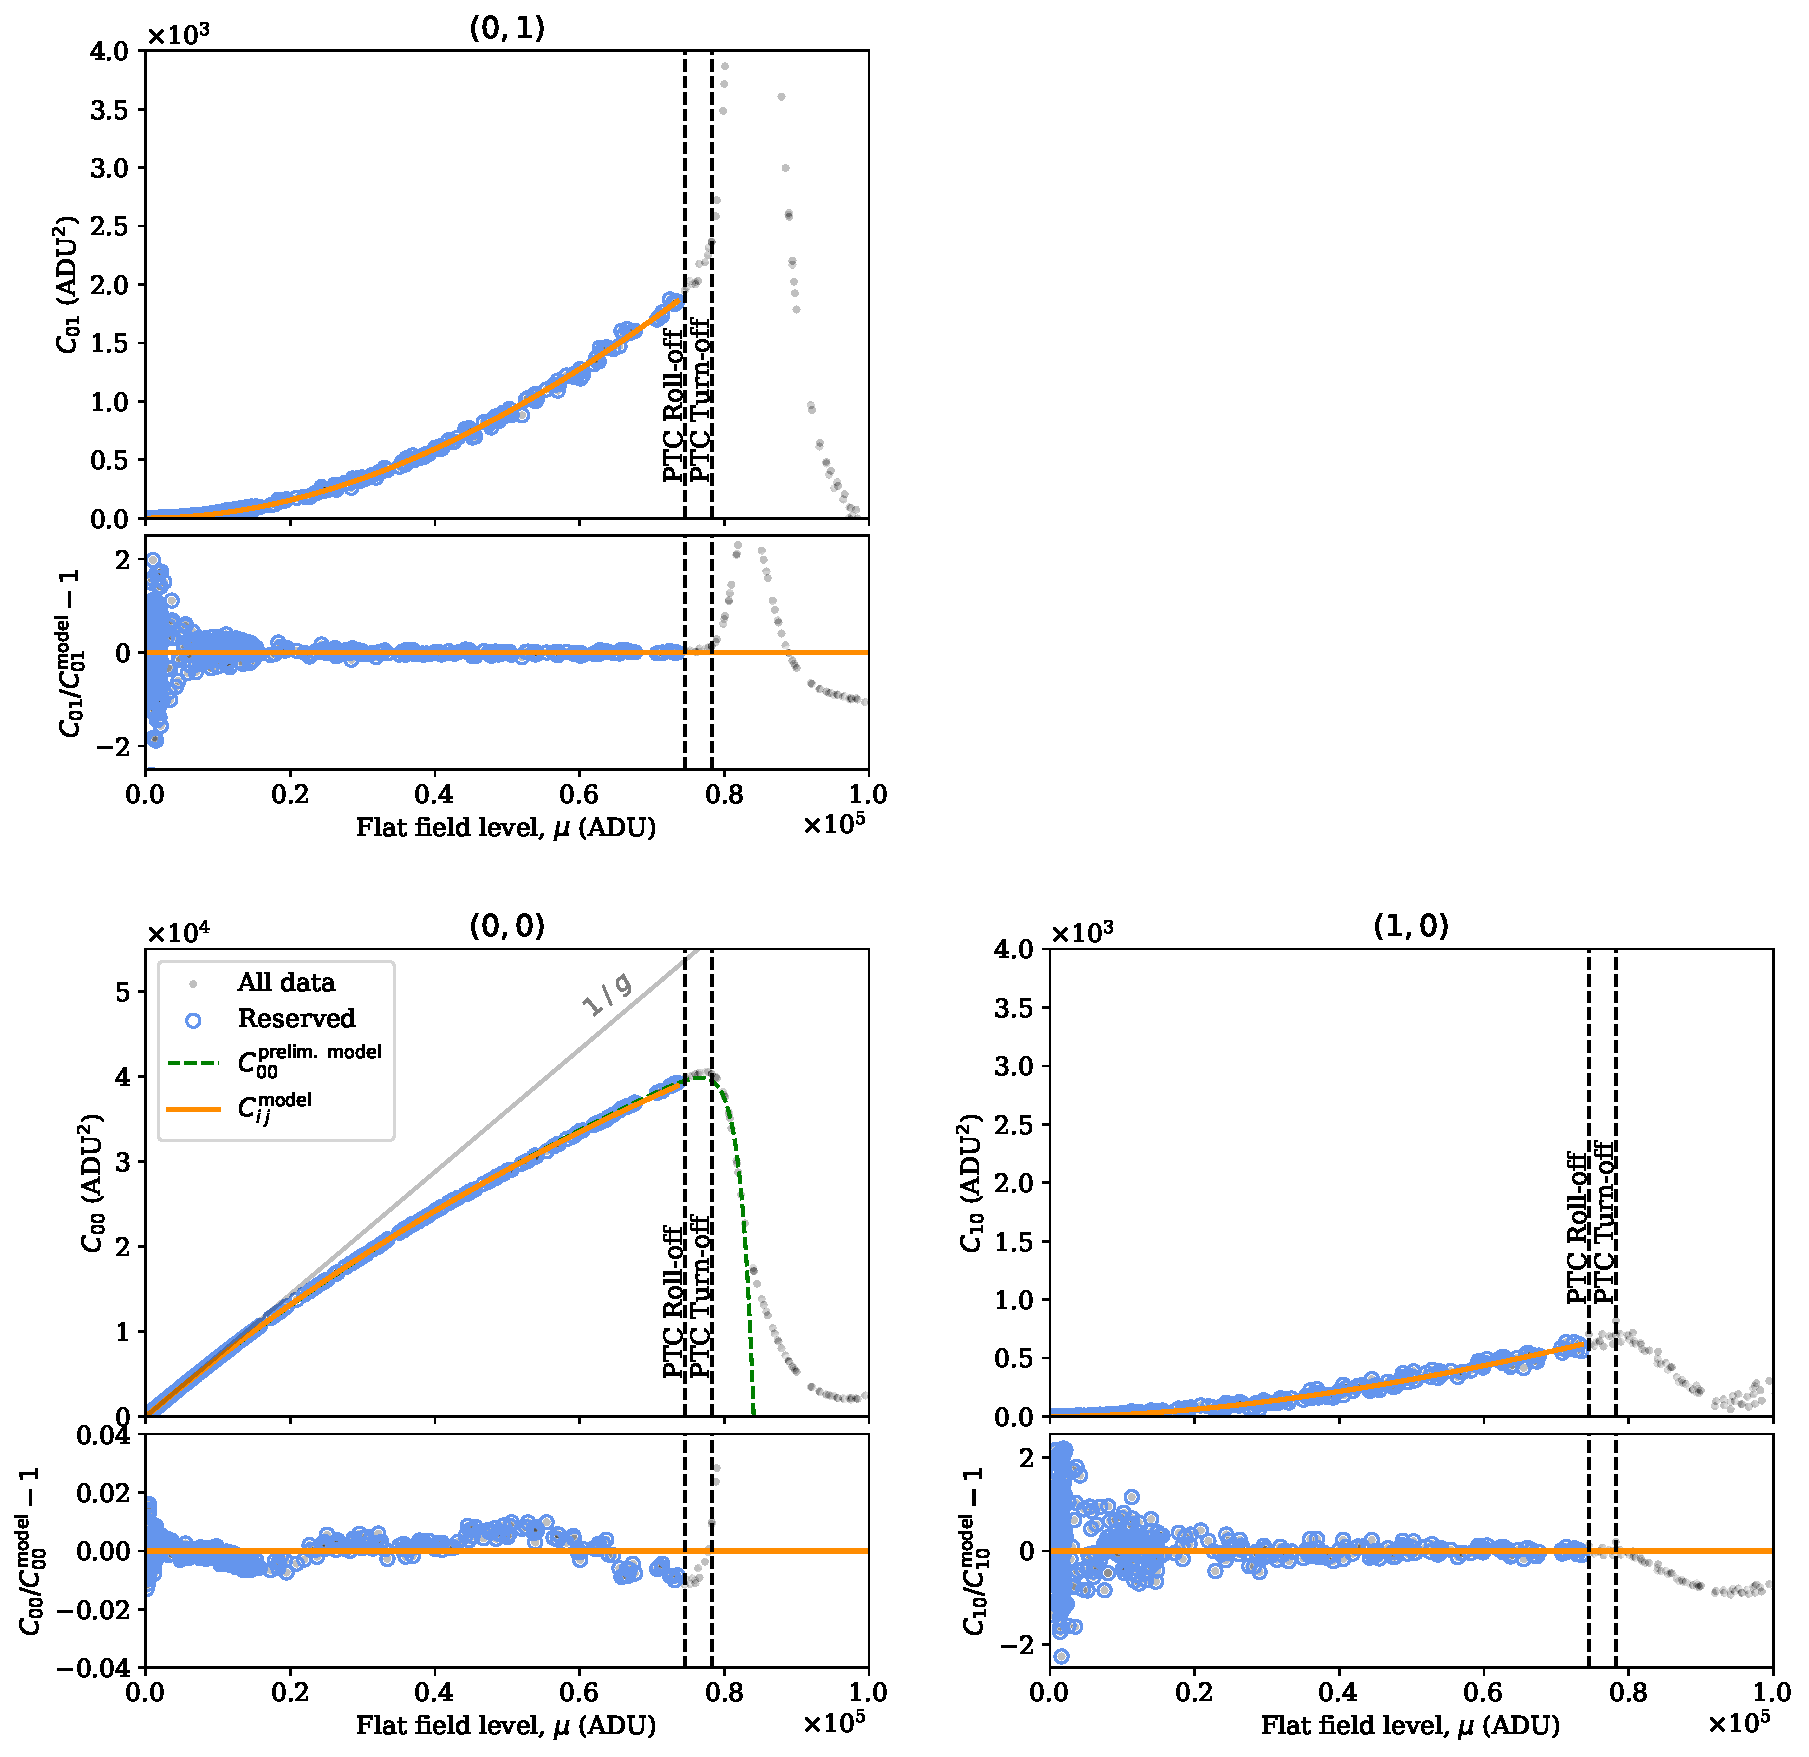
\includegraphics[width=\textwidth]{figures/ptc-triangle-det94-ampC03.pdf}
    \caption{Example PTC fit for amplifier~C03 on LSSTCam detector~94.
    Measured $C_{00}$ covariance points are compared to the preliminary fit (exponential approximation plus saturation roll-off) and the final full-covariance model variance.
    Vertical markers indicate the PTC rolloff and turnoff thresholds.}
    \label{fig:ptc-fit-example}
\end{figure*}

Because the gains are fit independently per amplifier, small fitting residuals can leave flux discontinuities at amplifier boundaries within a detector.
We add a subsequent step that measures the relative offsets between amplifiers in flat fields after gain correction and computes small adjustments to the gain to make the detector image continuous while preserving the average gain across the detector.
We compute the average gain adjustment in flat fields across a range of signal levels, and use these to produce overall ``adjusted gains''.
The adjustments to the gain are always small (less than 0.03), and uncorrelated between detectors.
These final gains are used for conversion of science images to electron units and construction of the variance plane for source detection.

The PTC calibration products are applied during instrument signature removal of science images in three ways.
First, the gain converts pixel values from ADU to electrons.
Second, the gain and read noise inform variance plane estimation.
Third, the saturated pixel mask flag (denoted ``SAT'') is set for all pixels with values greater than or equal to the PTC turnoff threshold.

% During science ISR, PTC-derived gains, variance-plane inputs, and saturation masking are applied at the steps shown in Figure~\ref{fig:isr-pipeline}; see \S\ref{sec:isr-science}.


\subsection{Brighter-Fatter Effect} \label{sec:processing:calibration:bf}

The brighter-fatter (BF) effect is the first influence the detector has on an incident signal (Figure~\ref{fig:detector-boxes}).
Accumulated electrons in a pixel repel incoming charges into neighboring pixels.
Brighter point sources therefore appear wider in the recorded images.
This electrostatic effect reduces to an effective change in pixel area and introduces correlations between nearby pixel values.
The effect is intrinsic to thick CCDs and can significantly bias point-spread-function (PSF) photometry and shape measurement.

The BF effect has been extensively characterized for LSSTCam by laboratory and in-dome commissioning measurements \citep{broughton2024}.
The strength of the effect is anisotropic ($a_{01}/a_{10} \sim 3$), long-ranged ($\sim 10$~px), and wavelength dependent.
It is also about twice as strong in the E2V-family detectors as in ITL-family detectors.

Several BF correction methods have been proposed and implemented in the LSST Science Pipelines \citep{gruen-2015,coulton-2018,astier-regnault-2023,broughton2024}, and they differ widely in their underlying assumptions.
\citet{broughton2024} found that modeling individual boundary shifts for every pixel (N, S, E, W) is required for adequate correction at the level needed for LSST Y10 science requirements.
Flat-field pixel correlations can measure only the net per-pixel area change, so determining these boundary shifts requires additional electrostatic modeling.
For processing raw images from DP2, we use the \citet{astier-regnault-2023} algorithm developed for Hyper Suprime-Cam, which derives from electrostatic physics and treats each pixel boundary individually.

% The correction assumes three simplifying conditions.
% First, the average charge current into a pixel is approximately constant during a long exposure, even when the PSF varies with time.
% Second, fourth-order terms in Eq.~\ref{eq:cov_model} are negligible; at the scale of the BF effect, the corresponding coefficients are of order $10^{-24}$.
% Third, photons convert to electrons quickly after entering the detector.
% Simulations and empirical modeling indicate that most photons in $u$ through $i$ bands convert within the top few microns of silicon, while the BF influence on charge drifting to the pixel bottom occurs primarily in the last several microns.
% Chromatic effects are therefore likely negligible for photons with wavelengths across the LSST bandpasses.

\begin{deluxetable}{ll}[t!]
    \tablecaption{Parameter Priors for the Electrostatic Brighter-Fatter Effect (BFE) Model Fit\label{tab:bf-electrostatic-fit-priors}}
    \tablehead{
        \colhead{Parameter} & \colhead{Prior}
    }
    \startdata
        Si thickness, $t$ ($\mu$m)        & $100$ (fixed) \\
        Pixel size, $p$ ($\mu$m)         & $10$ (fixed) \\
        Charge cloud height, $z_q$ ($\mu$m)      & $0 \leq z_q \leq t/2$ \\
        Charge cloud length, $a$ ($\mu$m)        & $10^{-5} \leq a \leq 0.35\,p$ \\
        Charge cloud width, $b$ ($\mu$m)         & $10^{-5} \leq b \leq 0.35\,p$ \\
        Potential well vertex height,\\horizontal $z_{sh}$ ($\mu$m)    & $0 \leq z_{sh} \leq t/2$ \\
        Potential well vertex height,\\vertical $z_{sv}$ ($\mu$m)    & $0 \leq z_{sv} \leq t/2$ \\
    \enddata
    \tablecomments{Priors on the fit parameters are informed by pixel-level simulations of the electric fields in these pixels \citep{Lage_2017}. The potential well vertices refer to the heights above the front-side of the CCD to the saddlepoints in the electric field that defines the pixel boundaries in the vertical (0, 1) and horizontal (1, 0) directions. The electrostatic model assumes that the stored charge cloud in the sensor takes the form of a flat, rectangular sheet of charge with length ($a$) and width ($b$). The inequality constraints $z_{sh} > z_q$, $z_{sv} > z_q$ are enforced during optimization, which is true in the unsaturated signal level regime.}
\end{deluxetable}

Calibration of the BFE using this algorithm takes the form of modeling a charge cloud at the bottom of a pixel, computing
how the effective areas of nearby pixels would be expected to change electrostatically in response. It adjusts some geometric parameters (summarized in Table~\ref{tab:bf-electrostatic-fit-priors}), and solves
Gauss's law to compute the shift of pixel boundaries and the relative change in pixel area from each shift ($\mathbf{a}^{\mathrm{N}}$,
$\mathbf{a}^{\mathrm{S}}$, $\mathbf{a}^{\mathrm{E}}$, $\mathbf{a}^{\mathrm{W}}$).
We optimize these parameters to best fit the
measured net pixel area changes ($\mathbf{a}$ from Eq.~\ref{eq:cov_model}):
\begin{equation}
    \mathbf{a} = \mathbf{a}^{\mathrm{N}} + \mathbf{a}^{\mathrm{S}} + \mathbf{a}^{\mathrm{E}} + \mathbf{a}^{\mathrm{W}}.
\end{equation}

In principle, the BFE can vary amplifier-to-amplifier, but we have observed only noise-level variations in the pixel distortion matrices across amplifiers and even detector families.
For this reason, and to avoid discontinuous amplifier boundaries, the fit is performed at the detector level.
All $a_{ij}$ matrices from well-behaved amplifiers are 3$\sigma$-clipped elementwise and averaged into a detector-mean $a_{ij}$; the scatter becomes the per-element uncertainty, and a single fit is run against this average pixel distortion matrix.
The output calibration data product is the set of model parameters and a model that can be evaluated per-detector.

Applying this calibration to remove the effect during ISR uses the boundary-shift matrices $\mathbf{a}^{\mathrm{N}}$, $\mathbf{a}^{\mathrm{S}}$, $\mathbf{a}^{\mathrm{E}}$, and $\mathbf{a}^{\mathrm{W}}$ to redistribute flux accordingly.
We tile these into two, $(2n+1)\times(2n+1)$, convolution kernels $K^{H}$ and $K^{V}$ for the horizontal and vertical shifts, respectively; we apply sign flips and edge adjustments so each matrix sums to zero.
These matrices need not be symmetric, which is more realistic per \citet{broughton2024}.
Figure~\ref{fig:ebf-kernels} shows an example pair of these kernels for amplifier~C03 on detector~94, illustrating the dipole-like, charge-conserving structure that redistributes flux across the vertical and horizontal pixel boundaries.

\begin{figure}[t]
    \centering
    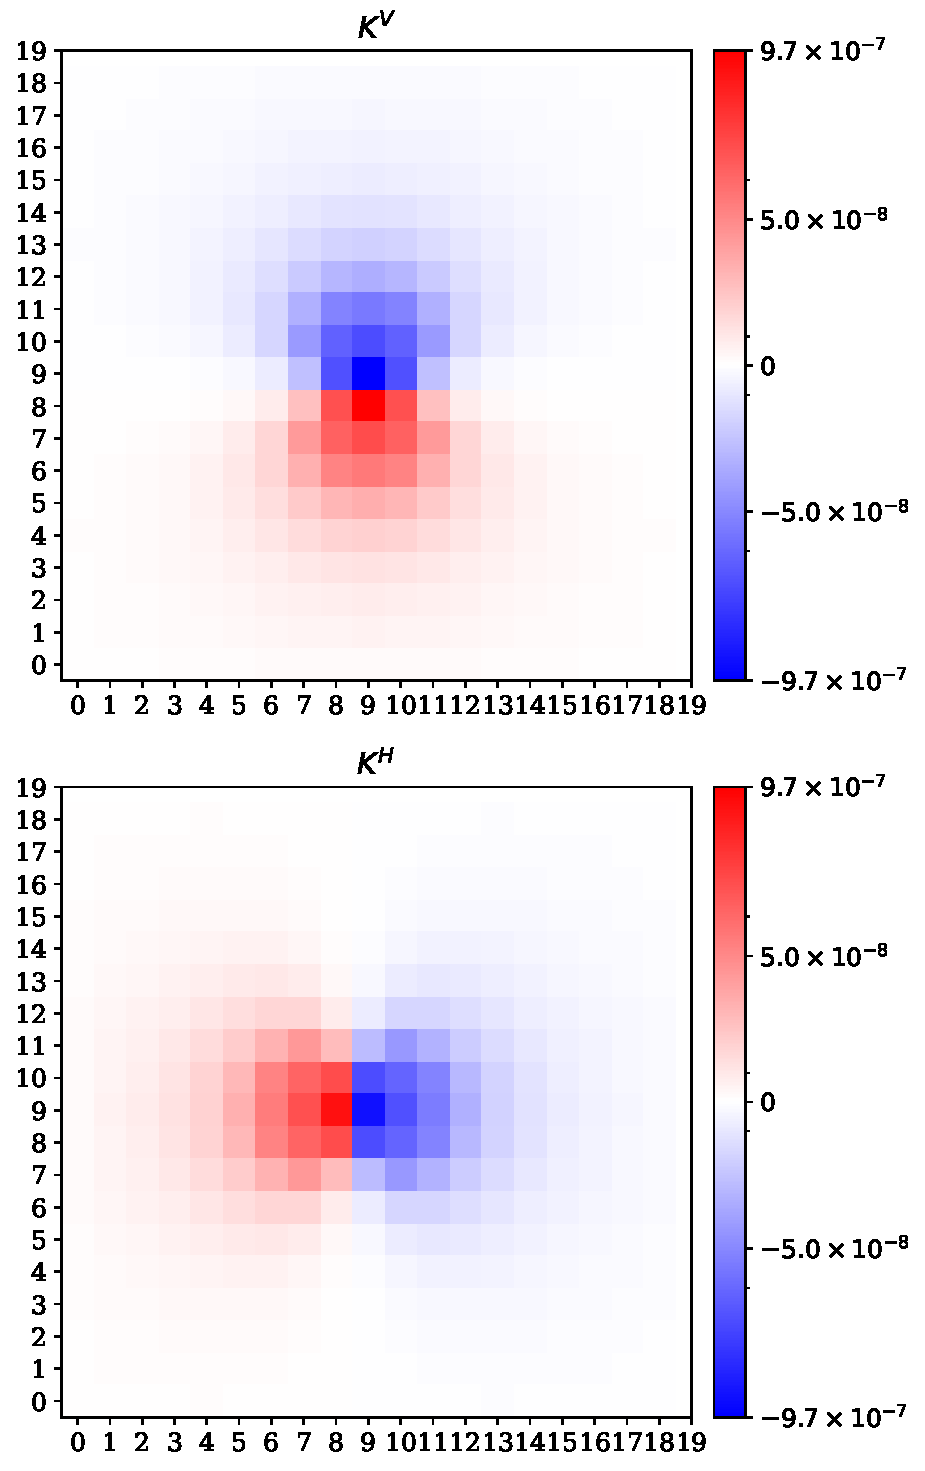
\includegraphics[width=\columnwidth]{figures/ebf-det94-ampC03-kVH.pdf}
    \caption{Example brighter-fatter correction kernels $K^{V}$ (vertical) and $K^{H}$ (horizontal) derived from the electrostatic BFE model for amplifier~C03 on LSSTCam detector~94.
    The diverging color scale shows the fractional charge redistributed across pixel boundaries; each kernel sums to zero to conserve charge and exhibits the antisymmetric dipole structure that moves flux from the brighter pixel to its neighbors.}
    \label{fig:ebf-kernels}
\end{figure}
For an image $Q_{ij}$ in natural gain-corrected units of electrons, the amount of charge lost over the vertical and horizontal boundaries is:
\begin{align}
    \delta^{H}_{ij} &= \tfrac{1}{2}\!\!\sum_{kl}\!\!K^{H}_{kl}\,Q_{i-k,\,j-l}, \notag \\
    \delta^{V}_{ij} &= \tfrac{1}{2}\!\!\sum_{kl}\!\!K^{V}_{kl}\,Q_{i-k,\,j-l},
    \label{eq:bf-shift}
\end{align}
The $1/2$ prefactor accounts for the average BFE assuming a constant rate of charge accumulation during an exposure.
The corrected image is assembled by removing the charge each pixel lost across its $N$/$E$ boundaries and adding what it gained from $S$/$W$ neighbors, guaranteeing charge conservation by construction, $\sum_{ij}Q^{\mathrm{corr}}_{ij}=\sum_{ij}Q_{ij}$.
This correction does not require iterative convolutions. Unlike the \citet{coulton-2018} algorithm used for DP1 \citep{2025rubn.rept...31N}, which requires multiple convolutions to reach convergence, we perform exactly two convolutions with the horizontal and vertical boundary-shift matrices.

% During science ISR, the brighter-fatter correction is applied at the step shown in Figure~\ref{fig:isr-pipeline}; see \S\ref{sec:isr-science}.


\subsection{Bias} \label{sec:processing:calibration:bias}

We describe how master biases are constructed (overscan handling, trimming, combination statistic, masking) and the metrics used to monitor time stability.

\subsection{Dark} \label{sec:processing:calibration:dark}

We describe how master darks are produced (scaling by exposure time, cosmic-ray rejection, hot pixel treatment) and how residual structures are assessed.

\subsection{Flats} \label{sec:processing:calibration:flats}

We describe how flat-field calibrations are created (illumination correction strategy, normalization conventions, handling fringing/stray light) and how uniformity is quantified.
